\appendix

\makeatletter
\renewcommand\chapter{\@startsection {chapter}{0}{\z@}%
                                   {-3.5ex \@plus -1ex \@minus -.2ex}%
                                   {2.3ex \@plus.2ex}%
                                   {\normalfont\Huge\bfseries}}
\makeatother

\chapter{Figures}

\pagebreak

\makeatletter
\renewcommand\chapter{\@startsection {section}{0}{\z@}%
                                   {-3.5ex \@plus -1ex \@minus -.2ex}%
                                   {2.3ex \@plus.2ex}%
                                   {\normalfont}}
\makeatother


\section{\boldmath Two components, $\tau_1 = 150$ps, $\tau_2=190$-$230$ps \unboldmath \label{t1-150}}
\vfill

\begin{minipage}{.5\linewidth}
    \centering
    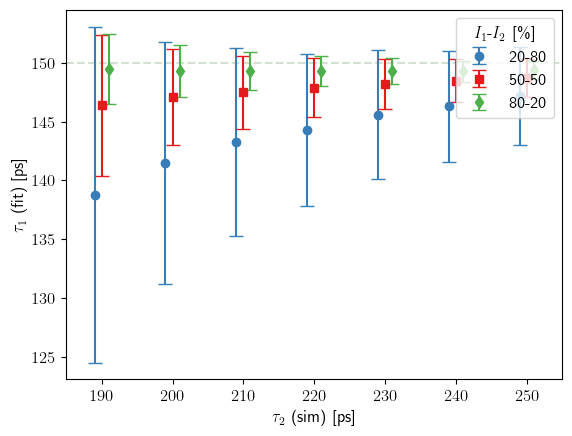
\includegraphics[width=\linewidth]{Batch 3/regular IRF/tau1 150/output/plotfin/t1.png}
    \captionof{figure}{Fitted $\tau_1$}
    \label{fig:150-t1}
\end{minipage}
\begin{minipage}{.5\linewidth}
    \centering
    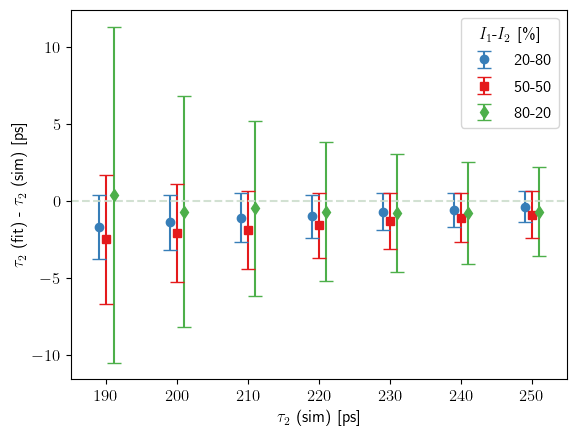
\includegraphics[width=\linewidth]{Batch 3/regular IRF/tau1 150/output/plotfin/t2.png}
    \captionof{figure}{$\tau_2$ (Fitted$-$Simulated)}
    \label{fig:150-t2}
\end{minipage}
\begin{minipage}{.5\linewidth}
    \centering
    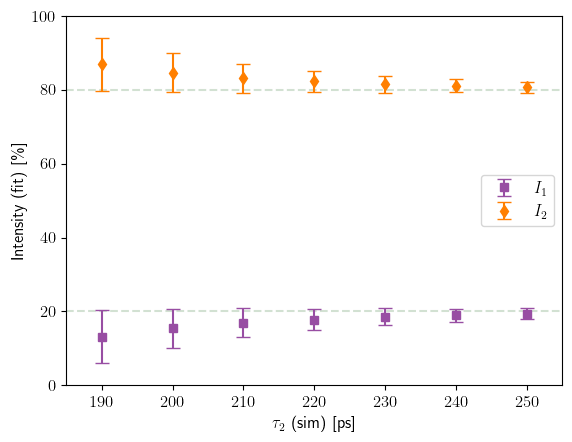
\includegraphics[width=\linewidth]{Batch 3/regular IRF/tau1 150/output/plotfin/2080.png}
    \captionof{figure}{$I_1 = 20\%, I_2 = 80\%$}
    \label{fig:150-2080}
\end{minipage}
\begin{minipage}{.5\linewidth}
    \centering
    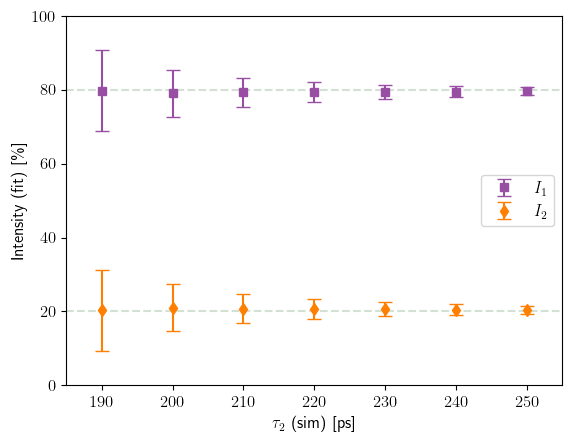
\includegraphics[width=\linewidth]{Batch 3/regular IRF/tau1 150/output/plotfin/8020.png}
    \captionof{figure}{$I_1 = 80\%, I_2 = 20\%$}
    \label{fig:150-8020}
\end{minipage}
\begin{minipage}{\linewidth}
    \centering
    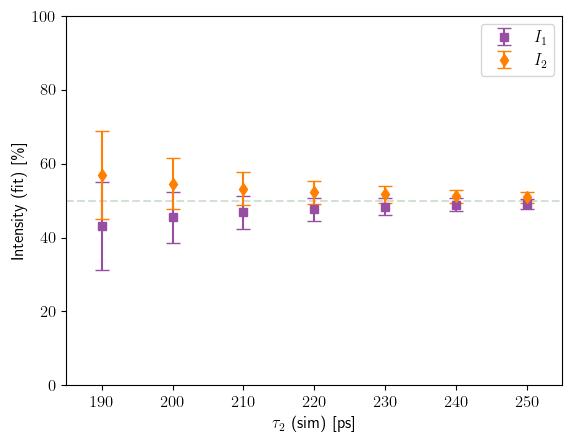
\includegraphics[width=.5\linewidth]{Batch 3/regular IRF/tau1 150/output/plotfin/5050.png}
    \captionof{figure}{$I_1 = 50\%, I_2 = 50\%$}
    \label{fig:150-5050}
\end{minipage}

\section{\boldmath Two components, $\tau_1 = 220$ps, $\tau_2=260$-$340$ps \unboldmath \label{t1-220}}
\vfill

\begin{minipage}{.5\linewidth}
    \centering
    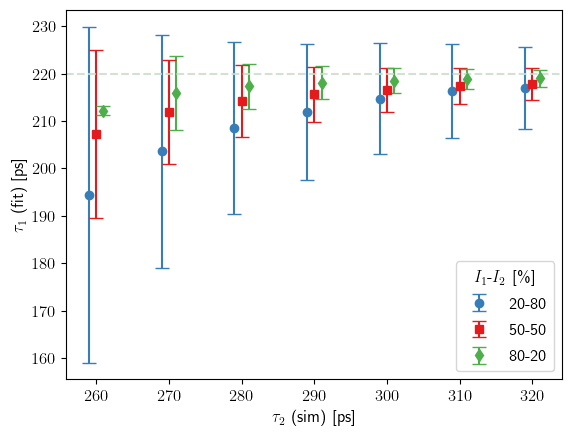
\includegraphics[width=\linewidth]{Batch 3/regular IRF/tau1 220/output/plotfin/t1.png}
    \captionof{figure}{Fitted $\tau_1$}
    \label{fig:220-t1}
\end{minipage}
\begin{minipage}{.5\linewidth}
    \centering
    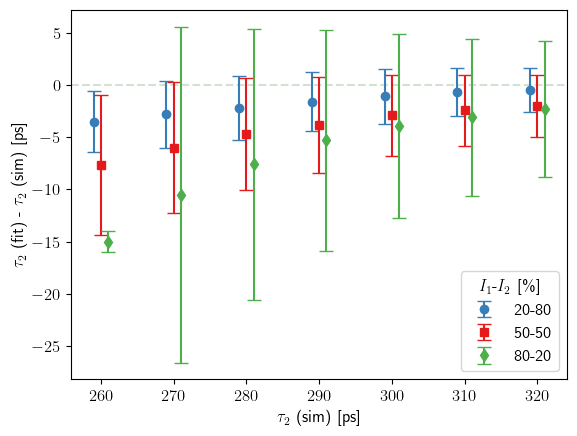
\includegraphics[width=\linewidth]{Batch 3/regular IRF/tau1 220/output/plotfin/t2.png}
    \captionof{figure}{$\tau_2$ (Fitted$-$Simulated)}
    \label{fig:220-t2}
\end{minipage}
\begin{minipage}{.5\linewidth}
    \centering
    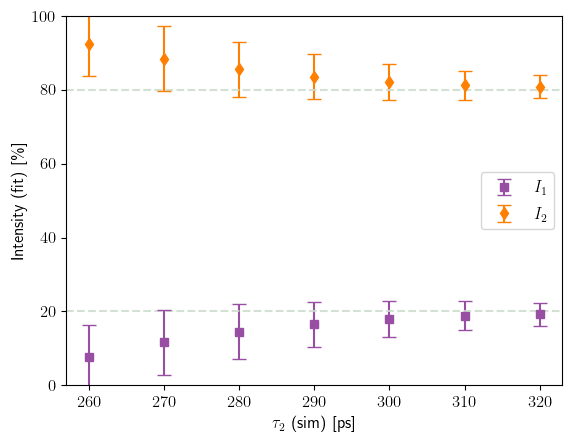
\includegraphics[width=\linewidth]{Batch 3/regular IRF/tau1 220/output/plotfin/2080.png}
    \captionof{figure}{$I_1 = 20\%, I_2 = 80\%$}
    \label{fig:220-2080}
\end{minipage}
\begin{minipage}{.5\linewidth}
    \centering
    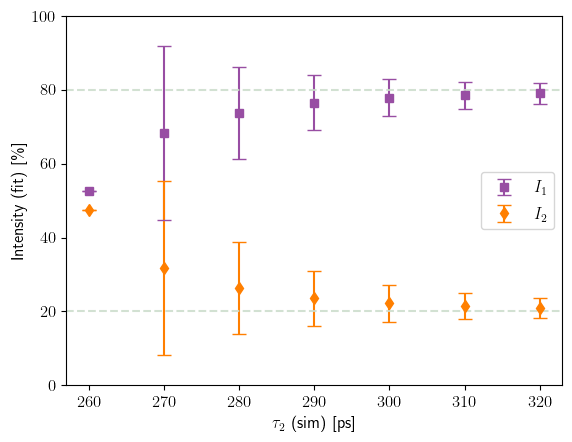
\includegraphics[width=\linewidth]{Batch 3/regular IRF/tau1 220/output/plotfin/8020.png}
    \captionof{figure}{$I_1 = 80\%, I_2 = 20\%$}
    \label{fig:220-8020}
\end{minipage}
\begin{minipage}{\linewidth}
    \centering
    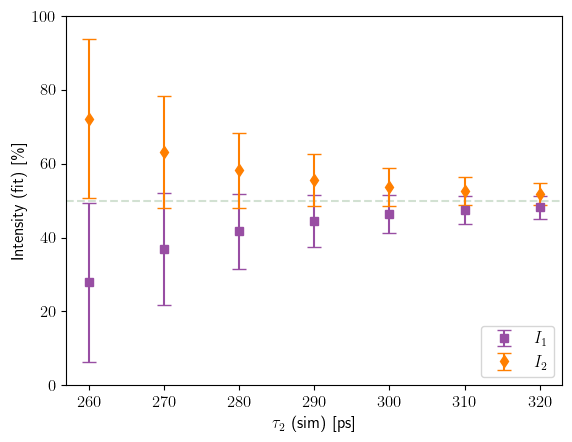
\includegraphics[width=.5\linewidth]{Batch 3/regular IRF/tau1 220/output/plotfin/5050.png}
    \captionof{figure}{$I_1 = 50\%, I_2 = 50\%$}
    \label{fig:220-5050}
\end{minipage}

\section{\boldmath Comparison two component fit, $\tau_1 = 150,180,220$ \unboldmath \label{comp-t1}}

\subsection*{\LARGE\centering\boldmath$\tau_1$\unboldmath}

\begin{minipage}{.47\linewidth}
    \centering
    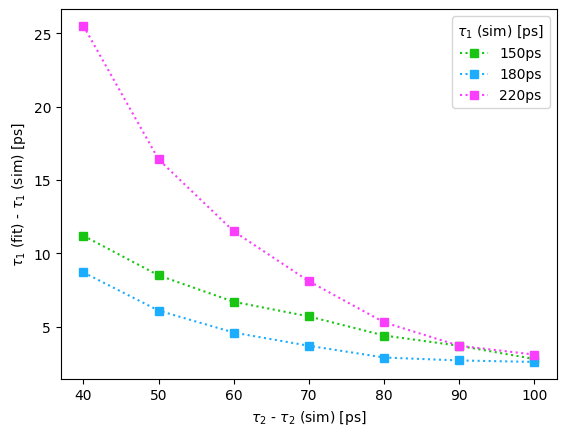
\includegraphics[width=\linewidth]{Batch 3/regular IRF/t1-diff 2080.png}
    \captionof{figure}{$I_1$-$I_2=20\%$-$80\%$}
    \label{fig:comp-t1-2080}
\end{minipage}
\hfill
\begin{minipage}{.47\linewidth}
    \centering
    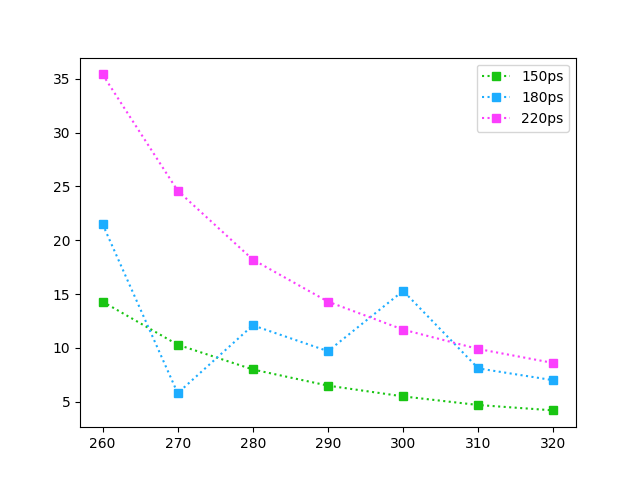
\includegraphics[width=\linewidth]{Batch 3/regular IRF/t1-err 2080.png}
    \captionof{figure}{Std. dev. $I_1$-$I_2=20\%$-$80\%$}
    \label{fig:comp-t1err-2080}
\end{minipage}
\begin{minipage}{.47\linewidth}
    \centering
    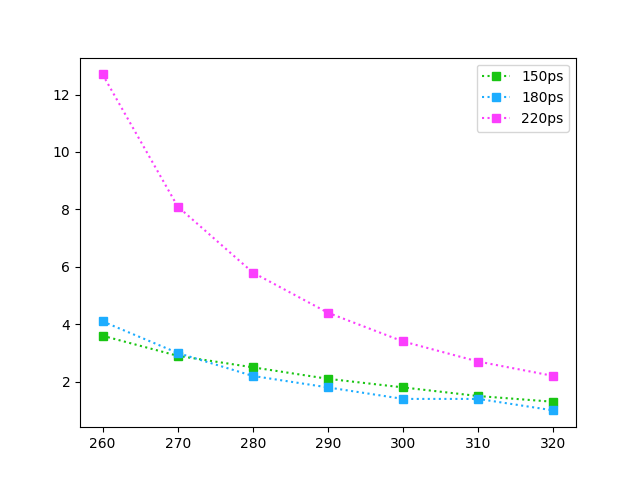
\includegraphics[width=\linewidth]{Batch 3/regular IRF/t1-diff 5050.png}
    \captionof{figure}{$I_1$-$I_2=50\%$-$50\%$}
    \label{fig:comp-t1-5050}
\end{minipage}
\hfill
\begin{minipage}{.47\linewidth}
    \centering
    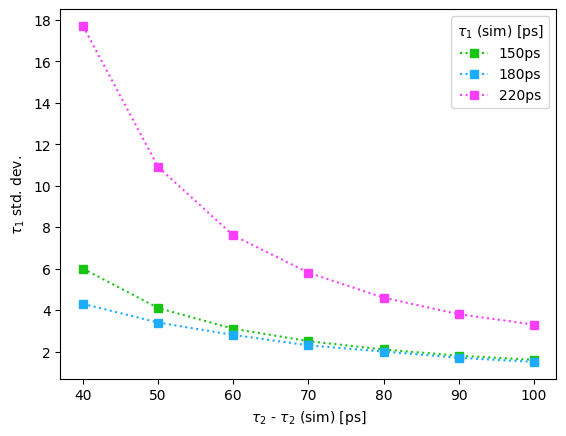
\includegraphics[width=\linewidth]{Batch 3/regular IRF/t1-err 5050.png}
    \captionof{figure}{Std. dev. $I_1$-$I_2=50\%$-$50\%$}
    \label{fig:comp-t1err-5050}
\end{minipage}
\begin{minipage}{.47\linewidth}
    \centering
    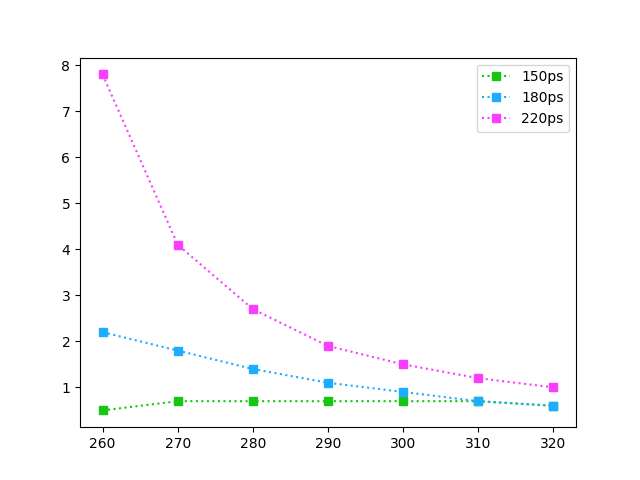
\includegraphics[width=\linewidth]{Batch 3/regular IRF/t1-diff 8020.png}
    \captionof{figure}{$I_1$-$I_2=80\%$-$20\%$}
    \label{fig:comp-t1-8020}
\end{minipage}
\hfill
\begin{minipage}{.47\linewidth}
    \centering
    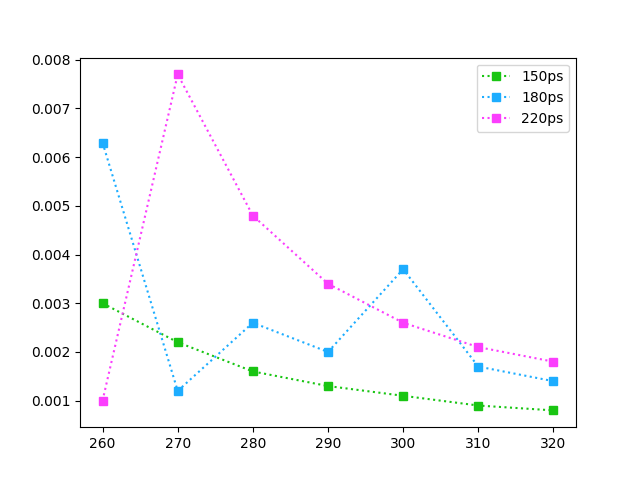
\includegraphics[width=\linewidth]{Batch 3/regular IRF/t1-err 8020.png}
    \captionof{figure}{Std. dev. $I_1$-$I_2=80\%$-$20\%$}
    \label{fig:comp-t1err-8020}
\end{minipage}

\vfill
\subsection*{\LARGE\centering\boldmath$\tau_2$\unboldmath}

\begin{minipage}{.5\linewidth}
    \centering
    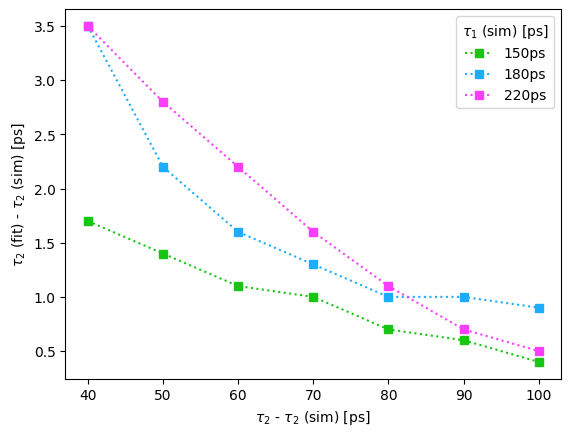
\includegraphics[width=\linewidth]{Batch 3/regular IRF/t2-diff 2080.png}
    \captionof{figure}{$I_1$-$I_2=20\%$-$80\%$}
    \label{fig:comp-t2-2080}
\end{minipage}
\begin{minipage}{.5\linewidth}
    \centering
    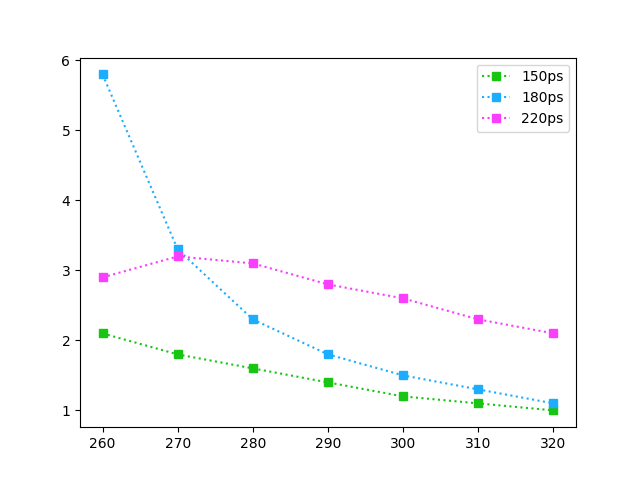
\includegraphics[width=\linewidth]{Batch 3/regular IRF/t2-err 2080.png}
    \captionof{figure}{Std. dev. $I_1$-$I_2=20\%$-$80\%$}
    \label{fig:comp-t2err-2080}
\end{minipage}
\begin{minipage}{.5\linewidth}
    \centering
    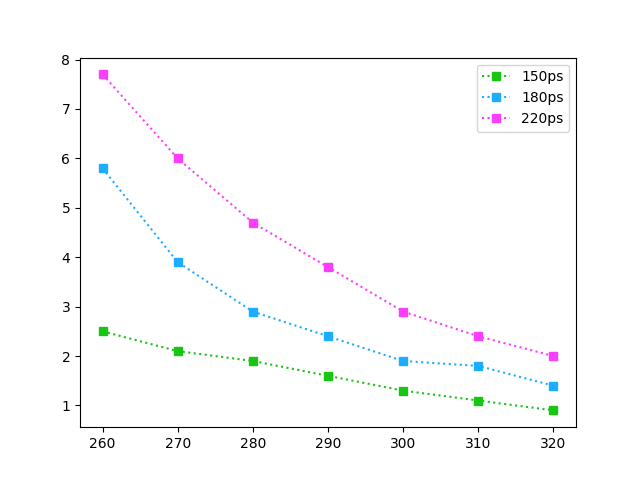
\includegraphics[width=\linewidth]{Batch 3/regular IRF/t2-diff 5050.png}
    \captionof{figure}{$I_1$-$I_2=50\%$-$50\%$}
    \label{fig:comp-t2-5050}
\end{minipage}
\begin{minipage}{.5\linewidth}
    \centering
    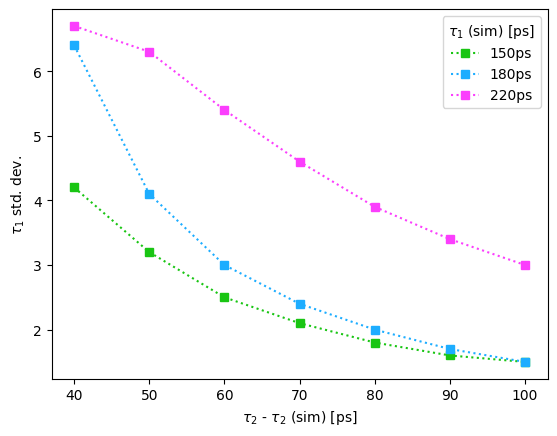
\includegraphics[width=\linewidth]{Batch 3/regular IRF/t2-err 5050.png}
    \captionof{figure}{Std. dev. $I_1$-$I_2=50\%$-$50\%$}
    \label{fig:comp-t2err-5050}
\end{minipage}
\begin{minipage}{.5\linewidth}
    \centering
    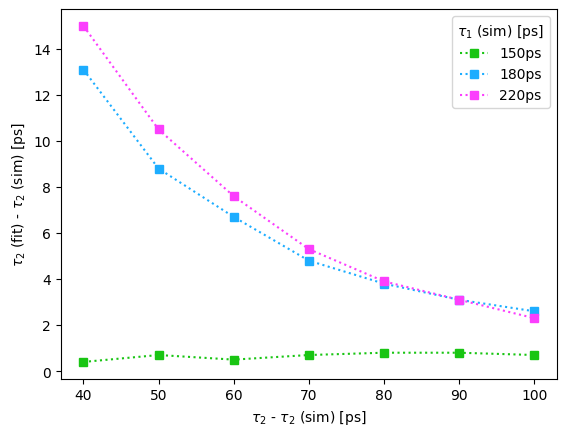
\includegraphics[width=\linewidth]{Batch 3/regular IRF/t2-diff 8020.png}
    \captionof{figure}{$I_1$-$I_2=80\%$-$20\%$}
    \label{fig:comp-t2-8020}
\end{minipage}
\begin{minipage}{.5\linewidth}
    \centering
    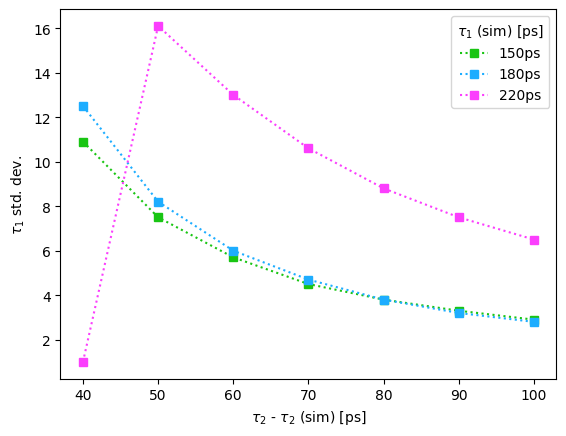
\includegraphics[width=\linewidth]{Batch 3/regular IRF/t2-err 8020.png}
    \captionof{figure}{Std. dev. $I_1$-$I_2=80\%$-$20\%$}
    \label{fig:comp-t2err-8020}
\end{minipage}

\vfill
\subsection*{\LARGE\centering Intensity}

\begin{minipage}{.5\linewidth}
    \centering
    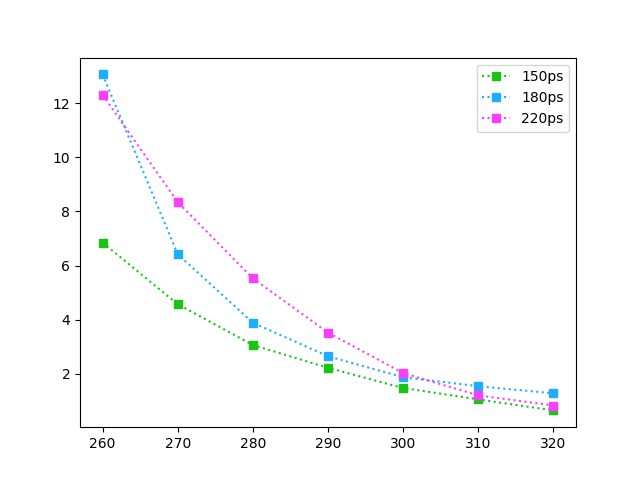
\includegraphics[width=\linewidth]{Batch 3/regular IRF/2080-diff i1.png}
    \captionof{figure}{$I_1$-$I_2=20\%$-$80\%$}
    \label{fig:comp-I-2080}
\end{minipage}
\begin{minipage}{.5\linewidth}
    \centering
    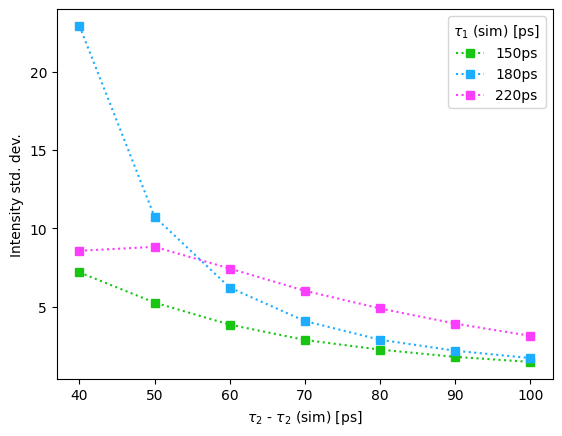
\includegraphics[width=\linewidth]{Batch 3/regular IRF/2080-err i1.png}
    \captionof{figure}{Std. dev. $I_1$-$I_2=20\%$-$80\%$}
    \label{fig:comp-Ierr-2080}
\end{minipage}
\begin{minipage}{.5\linewidth}
    \centering
    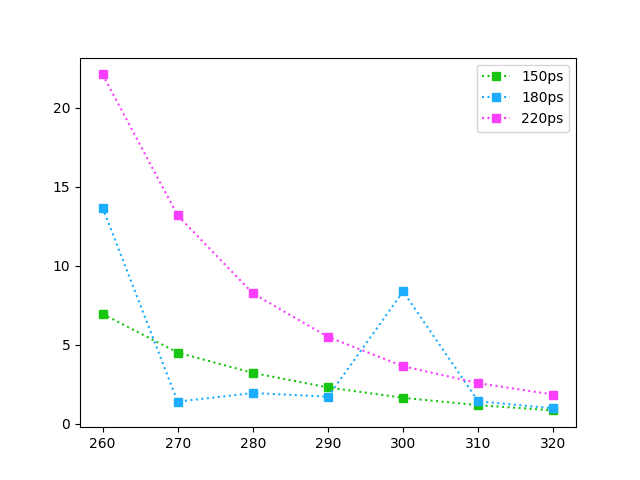
\includegraphics[width=\linewidth]{Batch 3/regular IRF/5050-diff i1.png}
    \captionof{figure}{$I_1$-$I_2=50\%$-$50\%$}
    \label{fig:comp-I-5050}
\end{minipage}
\begin{minipage}{.5\linewidth}
    \centering
    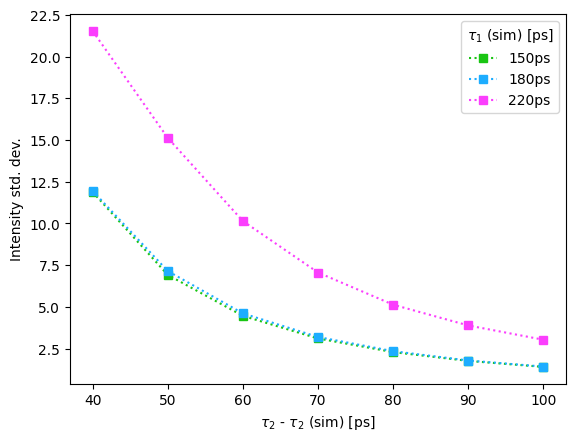
\includegraphics[width=\linewidth]{Batch 3/regular IRF/5050-err i1.png}
    \captionof{figure}{Std. dev. $I_1$-$I_2=50\%$-$50\%$}
    \label{fig:comp-Ierr-5050}
\end{minipage}
\begin{minipage}{.5\linewidth}
    \centering
    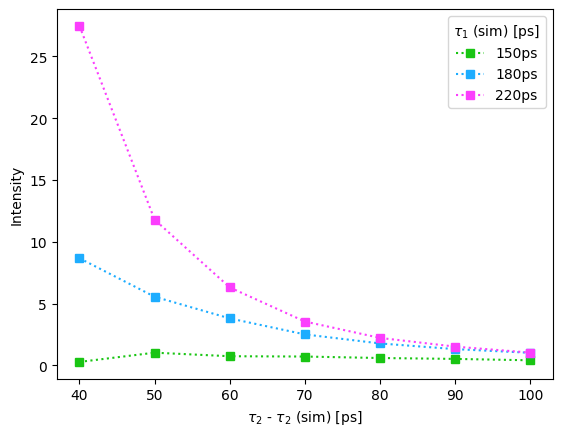
\includegraphics[width=\linewidth]{Batch 3/regular IRF/8020-diff i1.png}
    \captionof{figure}{$I_1$-$I_2=80\%$-$20\%$}
    \label{fig:comp-I-8020}
\end{minipage}
\begin{minipage}{.5\linewidth}
    \centering
    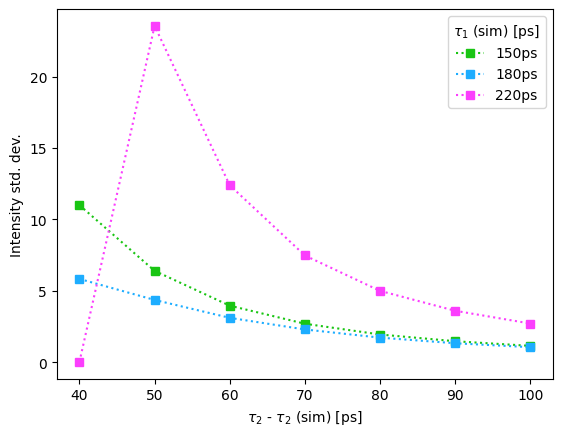
\includegraphics[width=\linewidth]{Batch 3/regular IRF/8020-err i1.png}
    \captionof{figure}{Std. dev. $I_1$-$I_2=80\%$-$20\%$}
    \label{fig:comp-Ierr-8020}
\end{minipage}